\chapter{Integration of rare processes}

\section{Muon pair production}

The process of muon pair production is a rare process with a negligible contribution to the overall energy loss of a propagated particle.
Although quantitatively negligible, the created signatures may be qualitatively relevant for neutrino observatories such as IceCube or underground detectors examining muons, see section \ref{sec:signatures} for a description of these signatures.

\subsection{Theoretical description}

Muon pair production describes the creation of a muon-antimuon pair by a particle in the field of an atomic nucleus $Z$, in case of an initial muon the reaction is
\begin{align*}
    \mu^- + Z \rightarrow \mu^- + \mu^+ + \mu^- + Z.
\end{align*}
A feynman diagram in leading order for the process is shown in figure \ref{fig:feynman_mupair}.

\begin{figure}
	\centering
	\input{content/feynman/feynman_mupair.tex}
    \caption{One possible feynman diagram describing the creation of a muon pair by an ingoing muon.}
    \label{fig:feynman_mupair}
\end{figure}

The process has been described in \cite{Kelner2000} where a simplified analytical double-differential cross section for muon pair production is given by
\begin{equation}
    \label{eqn:mupair}
    \frac{\mathrm{d}^2\sigma}{\mathrm{d}v \mathrm{d}\rho} = \frac{2}{3\pi} (Z \alpha r_\mu)^2 \frac{1-v}{v} \Phi(v, \rho) \ln \left( X \left(E, v, \rho \right) \right)
\end{equation}
with the relative energy loss $v$ and the asymmetry parameter $\rho$ defined by
\begin{align}
    v &= \frac{E_+ + E_-}{E}, & \rho &= \frac{E_+ - E_-}{E_+ + E_-}
\end{align}
and the energy of the produced (anti)muon $E_+$, $E_-$.
The functions $\Phi(v, \rho)$ and $X(E, v, \rho)$ have the form
\begin{align}
    \begin{split}
    \Phi(v, \rho) &= \left[ (2 + \rho^2) (1 + \beta) + \xi (3 + \rho^2) \right] \cdot \ln{ \left( 1 + \frac{1}{\xi} \right) }\\ &+ \left[ (1 + \rho^2) \left( 1 + \frac{3}{2} \beta \right) - \frac{1}{\xi} (1 + 2 \beta) (1 - \rho^2) \right] \cdot \ln{ (1 + \xi) }\\ &- 1 - 3 \rho^2 + \beta (1 - 2 \rho^2)
    \end{split}
\end{align}
where $X$ is given by
\begin{equation}
    X = 1 + U(E, v, \rho) - U(E, v, \rho_\text{max})
\end{equation}
with 
\begin{equation}
    U(E, v, \rho) = \frac{\frac{0.65 m_{\mu}}{m_e} A^{-0.27} B Z^{-\sfrac{1}{3}}}{1 + \frac{2 \sqrt{e} \mu^2 B Z^{-\sfrac{1}{3}} (1 + \xi) (1 + Y) }{m_e E v (1 - \rho^2)} }
\end{equation}
and with 
\begin{align}
    \xi &= \frac{v^2 (1 - \rho^2)}{4 (1 - v)}, & \beta &= \frac{v^2}{2 (1 - v)}, & Y &= 12 \sqrt{\frac{m_{\mu}}{E}}, & B &= 183.
\end{align}

The approximative expression \eqref{eqn:mupair} takes into account the finiteness of the nucleus as well as screening effects of the nucleus by atomic electrons.
A more precise formula for the differential cross section is given in \cite{Kelner2000} as well, however it includes multidimensional integrals that are hard to evaluate and is therefore not suited to be used here.
Furthermore, \eqref{eqn:mupair} is chosen to have a discrepancy compared to the precise formula of below $\SI{10}{\percent}$ for all $E > \SI{e4}{\mega\electronvolt}$, the discrepancy of the derived total cross section is even below $\SI{3}{\percent}$ for $E > \SI{3e4}{\mega\electronvolt}$.

The kinematic limits of the process for $v$ and $\rho$ are
%
\begin{align}
    v_\text{min} &= \frac{2 m_{\mu}}{E}, & v_\text{max} &= 1 - \frac{m}{E}, & \left| \rho \right| \leq \rho_{\text{max}} &= 1 - \frac{2 m_{\mu}}{v E},
\end{align}
%
for an initial particle with mass $m$ and are easy to retrace by demanding the condition that all particles involved have to fulfill $E > m_{\text{rest}}$ at all times.

\subsection{Implementation in PROPOSAL}
\label{sec:mupair_implementation}

% sloppypar is needed here because otherwise \texttt{...} breaks the layout because it cant use hyphenation here
\begin{sloppypar}
The process of muon pair production is implemented as an optional, additional interaction in PROPOSAL.
It is per default disabled in PROPOSAL and can be enabled by setting the keyword \texttt{mupair} in the configuration file to \texttt{MupairKelnerKokoulinPetrukhin} which is the parametrization that has been described in the previous section.
\end{sloppypar}

\begin{sloppypar}
To obtain the single-differential cross section in $v$ from \eqref{eqn:mupair}, a numerical integration across the entire kinematic range of $\rho$
%
\begin{equation}
    \frac{\symup{d}\sigma}{\symup{d}v} = \int_{\rho_{\text{min}}}^{\rho_{\text{max}}} \frac{\mathrm{d}^2\sigma}{\mathrm{d}v \mathrm{d}\rho} \, \symup{d}\rho
\end{equation}
%
is performed in PROPOSAL.
After sampling the relative energy loss $v$ during propagation according to \eqref{eqn:sample_v}, the asymmetry parameter $\rho$ is also sampled if the parameter \texttt{mupair\_particle\_output} has been set to \texttt{True}.
In this case, \eqref{eqn:mupair} is used with a fixed $v = v^{\ast}$ to solve the integral equation
\begin{equation}
    \left( \frac{\symup{d}\sigma}{\symup{d}v}(v^{\ast}) \right)^{-1} \int_{\rho_\text{min}}^{\rho} \frac{\mathrm{d}^2\sigma}{\mathrm{d}v \mathrm{d}\rho}(v^{\ast}) \, \symup{d}\rho = \xi
\end{equation}
for $\rho$ where $\xi \in \left[0,1\right)$ is a random number.
An additional random number is used to decide on the sign of $\rho$, the muon energies then assigned are $E_{\pm} = v E \cdot(1 \pm \rho)$.
In figure \ref{fig:rho_mupair}, the behavior of $\rho$ for different muon energies and different $v$ is shown.
For high energies, the process tends to have a higher asymmetry $\rho$, especially when a high relative energy loss is involved, while for lower energies, lower asymmetries are favored.
\end{sloppypar}

\begin{figure}
    \centering
    \includegraphics[scale=1]{build/mupair_rho.pdf}
    \caption{Histogram of $\lvert\rho\rvert$ for different $v$ of muons in ice. For each $v$, $\rho$ has been sampled $\num{e6}$ times. The dashed curves correspond to an initial muon energy of $E=\SI{e4}{\mega\electronvolt}$, the solid curves to $E = \SI{e9}{\mega\electronvolt}$.}
    \label{fig:rho_mupair}
\end{figure}

A comparison of the average energy loss in ice due to electron-positron pair production and muon pair production is shown in figure \ref{fig:dEdx_mupair}.
Both functions behave similarly as they both grow linearly with $E$, still the contribution from muon pair production is by about three orders of magnitudes lower for higher energies and even lower for small energies.
This observation shows that the process is negligible for the energy loss for the muon which is especially a result of the difference between the muon mass and the electron mass since 
\begin{align*}
	\frac{\sigma_{\mu \text{pair}}}{\sigma_{e \text{pair}}} \propto \frac{r_{\mu}^2}{r_e^2} \propto \frac{m_e^2}{m_{\mu}^2} \propto \num{2e-5}.
\end{align*}

\begin{figure}
    \centering
    \includegraphics[scale=1]{build/dEdx_mupair.pdf}
    \caption{Comparison of the average continuous energy losses of muons in ice due to electron-positron pair production and muon pair production. No energy cuts are applied in this plot, hence this plot represents the case where all losses are treated continuous.}
    \label{fig:dEdx_mupair}
\end{figure}

Figure \ref{fig:spectrum_mupair} shows a secondary particle spectrum where muon pair production is enabled.
The contribution for muon pair production tends to be distributed homogeneously but is, as expected, quantitatively negligible for all secondary energies.

\begin{figure}
    \centering
    \includegraphics[scale=1]{build/spectrum_mupair.pdf}
    \caption{Secondary particle spectrum for $\num{e5}$ muons with an initial energy of $\SI{e8}{\mega\electronvolt}$, propagated in ice. Muon pair production is enabled. The histogram shows the frequency of the stochastic losses during propagation, classified by the type of energy loss. The energy cuts applied here are $e_\text{cut} = \SI{500}{\mega\electronvolt}$, $v_\text{cut} = 0.05$.}
    \label{fig:spectrum_mupair}
\end{figure}

\subsection{Significant detector signatures}
\label{sec:signatures}

As already described and shown in section \ref{sec:mupair_implementation}, the contribution of muon pair production to the overall energy loss of muons is negligible.
However, for detectors interested in muon events, the effects of muon pair production may portray a source of significant signatures.
In the following, a group of muons moving into almost the same direction with only a small separation is called a muon bundle.
The origin of such a bundle can be muon pair production, in this case the bundle consists of three muons.

\subsubsection{IceCube detector}

Due to resolution effects, the IceCube detector is unable to identify the muons in a bundle as individual muon signatures.
However, the signature of a single muon traversing the detector is different from a muon bundle originating from muon pair production with the same sum of energy.
The signature of a high-energetic muon in IceCube is often characterized by a single high-energetic stochastic energy loss creating a spherical signature.
In a muon bundle, each muon with only a fraction of the total energy produces smaller stochastic losses.
Since the stochastic losses of the individual muons in the bundle are independent of each other, the resulting signature is homogeneous and the energy loss per distance of a bundle is more consistent compared to the energy loss per distance of a single muon with the same total energy. \todo{Include an event signature of a high-energetic muon and a muon bundle event? See Tomasz dissertation as a comparison.}

\subsubsection{Underground observatories}

Underground detectors observing muons originating from extensive air showers can use the information about muon bundles created in these air showers to learn about the cosmic ray composition and hadronic interaction models.
This is done by comparing the frequency and multiplicity of muon bundles as well as the muon separation measured in experiments with the predictions from Monte Carlo studies.
In \cite{MupairInRock}, the authors describe this procedure in more detail and point out a possible background from muon pair production.

While about $\SI{1}{\percent}$ to $\SI{10}{\percent}$ of the observed muons are part of muon bundles induced in the air shower, these bundles can also be produced due to muon pair production in rock or water above the underground detector.
According to calculations in \cite{MupairInRock}, these bundles induced by muon pair production can portray a background of up to $\SI{10}{\percent}$ compared to the conventional bundles in the showers, although more exact calculations have to be performed individually for each experiment with its own geometric properties.
Due to the difference in the distance between the creation and observation point of the muon bundle, both effects can be separated statistically by examining the separation distance in the bundle.
The separation of muon bundles due to muon pair production is mostly below $\SI{1}{\metre}$ while for muon bundles induced in air showers, only a small percentage of the muon bundles have such a small separation \cite{MupairInRock}.

\section{Weak interaction of charged leptons}

The process called weak interaction in PROPOSAL refers to the conversion of a charged lepton to a neutrino under exchange of a $W$-boson, i.e.\ a charged current weak interaction.
This interaction is highly suppressed compared to other processes, its signature however can be of importance, for example as a background for tau neutrino searches as described in section \ref{sec:weak_signature}.

\subsection{Theory and description of the data}
\label{sec:weak_theory}

The process of interest
%
\begin{equation}
    \label{eqn:weak_lepton}
    l + N \rightarrow \nu_l + X
\end{equation}
%
with a charged lepton $l$, the corresponding neutrino $\nu_l$, the initial nucleon $N$ and the hadronic final state $X$ describes the conversion of a charged lepton to a neutrino under exchange of a $W$-boson.
This specific process is related to the interaction of an anti-neutrino under exchange of a $W$ boson, i.e.\
%
\begin{equation}
    \label{eqn:weak_neutrino}
    \overline{\nu}_l + N \rightarrow \overline{l} + X,
\end{equation}
%
via crossing symmetry\footnote{The argument of crossing symmetry is identical when switching all particles with their corresponding antiparticles, i.e.\ the process $\overline{l} + N \rightarrow \overline{\nu}_l + X$ is connected to $\nu_l + N \rightarrow l + X$.} as depicted in figure \ref{fig:feynman_weak}.
%
\begin{figure}
    \centering
    \begin{tikzpicture}
  \centering
   % Sizes
   \pgfmathsetmacro{\len}{0.05cm}
   \pgfmathsetmacro{\halflen}{\len/4}
   \pgfmathsetmacro{\vertexsize}{\len/20}
   \begin{feynman}
       % vertices
       \vertex (a) at (-1*\len, 0.5*\len);
       \vertex (b) at (0, 0);
       \vertex (c) at (1*\len, 0.5*\len);
       \vertex (d) at (0, -1.5*\len);
       \vertex (e) at (-1*\len, -2*\len);
       \vertex (f) at (1*\len, -2*\len);

       \vertex (x) at (-0.4*\len, 0.5*\len);
       \vertex (y) at ( 0.4*\len, 0.5*\len); 
  
       % draw diagram
       \diagram* {
         (a) -- [anti fermion] (b) -- [anti fermion] (c),
         (b) -- [boson, edge label=\(W\)] (d),

       };
       \draw[thick, double] (e) -- (d) -- (f);
  
       \path[] (x) edge[<->, bend left] node [above] {crossing} (y);

       % labels
       \node[left] at (a) {$\overline{\nu}_{\mu}$};
       \node[right] at (c) {$\overline{\mu}$};
       \node[left] at (e) {$N$};
       \node[right] at (f) {$X$};

       % arrow inbetween

       \vertex (i1) at (1.6*\len, -0.75*\len);
       \vertex (i2) at (2.4*\len, -0.75*\len);
       \path[line width=0.8mm, black, ->, >=stealth] (i1) edge[->] node [] {} (i2);

       % vertices second diagram
       \vertex (a2) at (4*\len -1*\len, 0.5*\len);
       \vertex (b2) at (4*\len + 0, 0);
       \vertex (c2) at (4*\len + 1*\len, 0.5*\len);
       \vertex (d2) at (4*\len + 0, -1.5*\len);
       \vertex (e2) at (4*\len -1*\len, -2*\len);
       \vertex (f2) at (4*\len + 1*\len, -2*\len);
  
       % draw second diagram
       \diagram* {
         (a2) -- [fermion] (b2) -- [fermion] (c2),
         (b2) -- [boson, edge label=\(W\)] (d2),

       };
       \draw[thick, double] (e2) -- (d2) -- (f2);
  
       % labels second diagram
       \node[left] at (a2) {$\mu$};
       \node[right] at (c2) {$\nu_{\mu}$};
       \node[left] at (e2) {$N$};
       \node[right] at (f2) {$X$};

  \end{feynman}
\end{tikzpicture}
    \caption{Feynman diagrams of lepton interactions under exchange of a $W$-boson and its connection via crossing symmetry.}
    \label{fig:feynman_weak}
\end{figure}
%
Since the kinematics of both processes are identical, the differential cross sections are also identical except for a prefactor of $\sfrac{1}{2}$,
%
\begin{equation}
    \symup{d}\sigma\left( l + N \rightarrow \nu_l + X \right) = \frac{1}{2} \symup{d}\sigma\left( \overline{\nu}_l + N \rightarrow \overline{l} + X \right).
\end{equation}
%
Due to averaging over all possible initial states and summing over all possible final states when evaluating feynman diagrams, the prefactor $\sfrac{1}{2}$ must be taken into account since the muon can both be left-handed and right-handed while neutrinos are only observed in a left-handed state (and antineutrinos in a right-handed state).

Data on the differential cross section for the conversion of a neutrino to a charged lepton, i.e.\ the process \eqref{eqn:weak_neutrino}, are available from \cite{Cooper_Sarkar_2011}.
By using crossing symmetry, these data can directly be used to describe the conversion of a charged lepton to a neutrino, i.e.\ \eqref{eqn:weak_lepton}, which is the process of interest in PROPOSAL.

The cross sections for interactions of leptons with hadrons can be derived under the use of parton distribution functions which describe the probability to find a specific parton (quark or gluon) with a given fraction $x$ of the nucleon's momentum when the momentum transfer is given by $Q^2$.
To make predictions for the (anti)neutrino charged current cross sections, \cite{Cooper_Sarkar_2011} performs next-to-leading order calculations and uses the HERAPDF1.5 data set which provides the parton distribution functions based on deep-inelastic scattering measurements performed from 2003 to 2007 at the HERA experiment \cite{am2010proton}.

The values for $\sfrac{\symup{d}\sigma}{\symup{d}v}$ are provided as two-dimensional tables in $E$ and $v$ with $\num{100}$ entries in $E$ and, for each energy, $\num{110}$ entires in $v$.  
Here, $v$ describes the fraction of the initial lepton energy $E$ lost to the nucleon.
Tables are available for an ingoing neutrino or an ingoing antineutrino and for a proton or a neutron as a nucleon involved in the interaction.
The ranges are $\SI{10}{\giga\electronvolt} \leq E \leq \SI{e12}{\giga\electronvolt}$ and $v_\text{min} < v < 1$ with logarithmic steps in between where the lower limit of $v$ has been set to
%
\begin{align}
    v_\text{min} &= \frac{Q^2_{\text{min}}}{s}, & s &= 2 E m + m^2, & Q^2_{\text{min}} &= \SI{1}{\giga\electronvolt^2}
\end{align}
%
with the mass of the involved nucleon $m$ and the center-of-mass energy $\sqrt{s}$.
For values where $Q^2 < Q_\text{min}^2$, the underlying theory of quantum chromodynamics can not be treated perturbatively anymore, meaning that the predictions for the cross sections are not reliable in this kinematic range. 

\subsection{Implementation in PROPOSAL}

% sloppypar is needed here because otherwise \texttt{...} breaks the layout because it cant use hyphenation here
\begin{sloppypar}
The weak interaction process is by default disabled in PROPOSAL and can optionally be enabled by setting the keyword \texttt{weak} in the configuration file to \texttt{CooperSarkarMertsch} which is the parametrization described in the previous section.
\end{sloppypar}
For a component with an atomic number $Z$ and a mass number $A$, the differential cross section is combined from the given tables to be
%
\begin{equation}
	\frac{\symup{d}\sigma}{\symup{d}v} \propto Z \cdot \frac{\symup{d}\sigma_p}{\symup{d}v} + (A - Z) \cdot \frac{\symup{d}\sigma_n}{\symup{d}v}
\end{equation}
%
where the subscript refers to the nucleon involved in the interaction ($p$ for proton and $n$ for neutron).
PROPOSAL then uses a two-dimensional interpolation routine to obtain a continuous differential cross section from the discrete tables values.

In contrast to previously described processes, the weak interaction is a catastrophic loss meaning that the initial particle ceases to exist since it is converted to a different type of particle during the interaction.
Treating a process with this signature continuously as described in section \ref{sec:energy_loss_calculation} would therefore be unphysical.
Instead, all interactions with catastrophic losses are treated stochastically by setting $v_{\text{min}} = v_{\text{cut}}$ in \eqref{eqn:fE}, \eqref{eqn:stoch_crosssection} and \eqref{eqn:sample_v}.
Afterwards, PROPOSAL returns the produced neutrino as well as the energy transfer to the nucleon and stops the particle propagation.

\begin{figure}
    \centering
    \includegraphics[scale=1]{build/dNdx_weak.pdf}
    \caption{Comparison of the stochastic cross sections for muons in ice for weak interaction in comparison to other interactions. The cut settings are set to $e_\text{cut} = \SI{500}{\mega\electronvolt}$, $v_\text{cut} = 0.05$. Note that the weak interaction cross section is not affected by the cut settings.}
    \label{fig:dNdx_weak}
\end{figure}

Figure \ref{fig:dNdx_weak} shows the weak interaction cross section of muons in ice compared to the total stochastic cross section of default processes.
It is important to note for this comparison that, while $v_{\text{min}} = v_{\text{cut}}$ is used for the weak interaction, a regular energy cut of $e_\text{cut} = \SI{500}{\mega\electronvolt}$ and $v_\text{cut} = 0.05$ is still used for the other parametrizations.
Still, it becomes obvious that the weak interaction is a strongly suppressed process compared to all other interactions.

\subsection{Significant detector signatures}
\label{sec:weak_signature}

As described in the previous section, the weak interaction process is highly suppressed and therefore negligible in its contribution to the energy loss of a charged lepton.
However, under certain conditions, the detector signature of the process could be significant for searches of tau neutrinos, for example in the IceCube neutrino observatory.

\begin{figure}
    \centering
    \begin{subfigure}{0.46\textwidth}
        \centering
        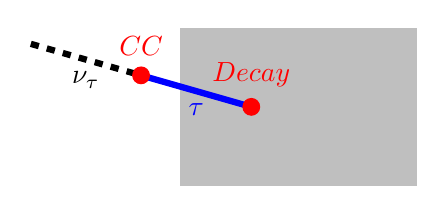
\begin{tikzpicture}
	\centering
	\fill [lightgray] (0.0, 0.0) rectangle (3.0, 2.0);
	\draw [line width=0.8mm, blue] (-0.5, 1.4) -- node[below] {$\tau$}  (0.9, 1.);
	\draw [line width=0.8mm, black, dashed] (-1.9, 1.8) -- node[below] {$\nu_{\tau}$}  (-0.5, 1.4);
	\draw[red,fill=red] (0.9, 1.) circle (0.7ex) node[label=above: $\scriptsize \text{Decay}$]{};
	\draw[red,fill=red] (-0.5, 1.4) circle (0.7ex) node[label=above: $\scriptsize \text{CC}$]{};
\end{tikzpicture} 

        \caption{Lollipop signature triggered by a tau neutrino.}
        \label{fig:lollipop_signature}
    \end{subfigure}%
    \hspace{0.06\textwidth}%
    \begin{subfigure}{0.46\textwidth}
        \centering
        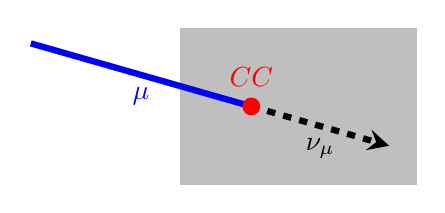
\begin{tikzpicture}
	\centering 
	\fill [lightgray] (0.0, 0.0) rectangle (3.0, 2.0);
	\draw [line width=0.8mm, blue] (-1.9, 1.8) -- node[below] {$\mu$}  (0.9, 1.);
	\draw [line width=0.8mm, black, dashed, ->, >=stealth] (0.9, 1.) -- node[below] {$\nu_{\mu}$}  (0.9+1.4+0.35, 1. - 0.4 - 0.1);
	\draw[red,fill=red] (0.9, 1.) circle (0.7ex) node[label=above: $\scriptsize \text{CC}$]{};
\end{tikzpicture} 

        \caption{Signature of a muon weakly interacting inside the detector.}
        \label{fig:weak_signature}
    \end{subfigure}
    \caption{Illustrations of two signatures relevant for tau neutrino searches. The detector volume is drawn gray, hadronic cascades are drawn as a red dot, observable tracks are drawn as blue lines and tracks that are not directly observable are drawn as a black, dotted line.}
    \label{fig:test}
\end{figure}

One possible signature hinting at a tau neutrino event called the "lollipop" signature is illustrated in figure \ref{fig:lollipop_signature}.
Here, a tau neutrino moving towards the detector interacts via a charged current before it reaches the detector and is being converted to a tau lepton.
The tau lepton then enters the detector, leaving behind an observable track of Cherenkov light emerging from the tau itself and the created secondary particles.
Due to its short lifetime, the created tau can only reach the detector if its energy is high enough, the average tau decay length scales with energy as \SI{5}{\cm\per\tera\electronvolt} \cite{Aartsen_2016} meaning the tau energy has to be $E_{\tau} \gtrapprox \SI{100}{\tera\electronvolt}$.
If the tau decays to a hadron inside the detector, a hadronic cascade is generated at the end of the track, giving the signature its characteristic name. 

This tau neutrino signature can be imitated by the event shown in figure \ref{fig:weak_signature}.
In this case, a muon, leaving behind a track, enters the detector where it weakly interacts and is therefore converted to a neutrino.
Due to the energy transfer to the involved nucleus in the weak interaction, the process creates a hadronic cascade comparable to the cascade of a hadronic tau decay.
Since the created neutrino is not observable, the overall signature where a track starts outside the detector and ends in a hadronic cascade can be confused with the lollipop signature from figure \ref{fig:lollipop_signature}.
However, the tracks from both signatures behave differently since the energy loss per distance of a muon is higher than the energy loss of a tau.
To have a similar track signature, the tau involved needs to have an energy that is about $\num{6}$ to $\num{11}$ times higher than the energy of a corresponding muon \cite{Sandrock:2018hpj}.

It follows that analyses searching for lollipop signatures have to consider the weak interaction as a possible background.
According to approximative calculations in \cite{Sandrock:2018hpj} based on the properties of the IceCube detector, the expected rate of false lollipop events due to atmospheric muons undergoing weak interaction is about $\SI{2e-2}{\per yr}$. 
This, together with further approximative calculations for real lollipop signatures from tau neutrino events, corresponds to a possible background of $\SI{10}{\percent}$.
However, further effects such as event selection efficiency (assumed to be perfect in this calculation) or a detailed detector simulation were not taken into account but need to be evaluated when conducting a detailed analysis.
